\chapter{Data}
\label{ch:data}

\section{Monte Carlo Simulations}
\label{sec:mc_simluation}
As training data for various neural network models, we do not use measured data by the ATLAS detector, but rather \emph{simulated events}. 
Simulations are based on physical models, detector models, and stochastic processes involved in both the physics and the detector.
Hence the name, \MC simulations.

Simulation can be split into two parts: the physics simulation and the detector simulation.
The physical part uses the \texttt{Pythia 8.2} package \cite{pythia}, a state-of-the-art event generator.
The detector response is made using the \texttt{Geant4} package \cite{geant4} tailored to the ATLAS detector \cite{atlas_sym}.

After the simulations, the \MC data comes in the same format as the actual data from the detector.
For the simulation to make physical sense, they assign \emph{weight} to each event based on the cross section of the simulated process.
The only difference is that the \MC data contains \emph{truth information} from the physical simulation, which is used to train the neural networks.
However, object reconstruction is still done the same way as for the actual data.
Jet reconstruction is done in two steps: first, the jet constituents are identified, and then the jet is reconstructed from the constituents. 
Constituent identification will be discussed in \cref{sec:pfo} and jet reconstruction in \cref{sec:jet_reco}.

\section{Event Production}
\label{sec:event_production}
\texttt{Pythia} is capable of simulating hard interactions at LO (leading order in perturbative QCD) accuracy and clustering partons into hadrons using the Lund string model (described in \cref{sec:hadronization}).
We utilize the ATLAS A14 tuned parameters \cite{atlas_A14_tunes} using the \texttt{NNPDF23LO} \cite{NNPDF23LO} parton density functions (see \cref{sec:hadronization}).
The decays of heavy flavor hadrons are simulated using the \texttt{EvtGen} package \cite{EvtGen}.

Cross sections of events depend highly on the $\pT$ of scattered partons. 
To be able to describe well the high $\pT$ (low probability, i.e., cross section) events, the \MC \texttt{Pythia} production is split into \texttt{JZ} slices. 
Each slice has a different $\pT$ range of leading (with the highest $\pT$) jet.
In the original dataset are 13 slices, \texttt{JZ0}-\texttt{JZ12}, but we will only utilize \texttt{JZ1}-\texttt{JZ5}, which are the most interesting for physical analyses.
A summary of the used \texttt{JZ} samples is shown in \cref{tab:jz}. 
To make the physical sense of the \texttt{JZ} slices, each slice is assigned a cross section on top of the event weight, also summarized in \cref{tab:jz}.
\begin{table}[!htb]
    \centering
    \caption{Summary of the used \texttt{JZ} samples. Each slice corresponds to a different $\pT$ range of the leading jet. The higher the $\pT$ the lower the probability, i.e. cross section $\sigma$.}
    \label{tab:jz}
    \begin{tabular}{ccccc}
    \toprule
        Slice & $\pT$ range [GeV] & $\sigma$ [nb] & Filter Efficiency & Size [GB] \\
    \midrule
        \texttt{JZ1} & 20-60 & $7.8\cdot10^{10}$ & $2.44\cdot10^{-2}$ & 78    \\
        \texttt{JZ2} & 60-160 & $2.4\cdot10^{9}$ & $9.86\cdot10^{-3}$ & 29    \\
        \texttt{JZ3} & 160-400 & $2.6\cdot10^{7}$ & $1.16\cdot10^{-2}$ & 70    \\
        \texttt{JZ4} & 400-800 & $2.5\cdot10^{5}$ & $1.34\cdot10^{-2}$ & 39    \\
        \texttt{JZ5} & 800-1300 & $4.6\cdot10^{3}$ & $1.45\cdot10^{-2}$ & 22    \\
    \bottomrule
    \end{tabular}
\end{table}




% 7.8e+10 * 0.0244 = 1.9e+8
% 2.4e+9 * 0.00986 = 2.4e+6
% 2.6e+7 * 0.0116 = 3e+5
% 2.5e+5 * 0.0134 = 3.3e+3
% 4.6e+3 * 0.0145 = 6.6e+1
% sum = 2.1e+8
% relative 
% 1.9e+8 / 2.1e+8 = 0.9
% 2.4e+6 / 2.1e+8 = 0.01
% 3e+5 / 2.1e+8 = 0.0014
% 3.3e+3 / 2.1e+8 = 0.00016
% 6.6e+1 / 2.1e+8 = 0.0000032















\red{[???? ADD INFO ABOUT \emph{PartonTruthLabelID}, SEE \url{https://acode-browser.usatlas.bnl.gov/lxr/source/athena/PhysicsAnalysis/AnalysisCommon/ParticleJetTools/Root/JetPartonTruthLabel.cxx} AND \url{https://twiki.cern.ch/twiki/bin/view/AtlasProtected/Run2JetMoments\#Jet_attributes_for_Run_2}]}

\section{Constituent Identification}
\label{sec:pfo}
Our study identifies jet constituents using the \PFa \cite{PFO}.

The \PFa is based on the Topocluster algorithm \cite{topocluster}, which uses only calorimeter (electromagnetic and hadron) information to identify energy clusters.
The seed of the cluster is a signal of strength at least $4\sigma$, where $\sigma$ is the noise of the calorimeter.
When such a seed is found, the algorithm searches for neighboring cells with signal strength above $2\sigma$.
The neighboring cells are added to the cluster, and the algorithm repeats the search for other neighboring cells.
When no more neighboring cells with signal $>2\sigma$ are found, all cells that form a boundary are added to the cluster.
After the algorithm looks for local maxima in the cluster and splits it into two or more, if necessary.
If a cell is neighboring two or more clusters, the cell is assigned to two clusters with the highest energy.
An example of clusters is shown in \cref{fig:topocluster}. 
\begin{figure}[ht]
    \centering
    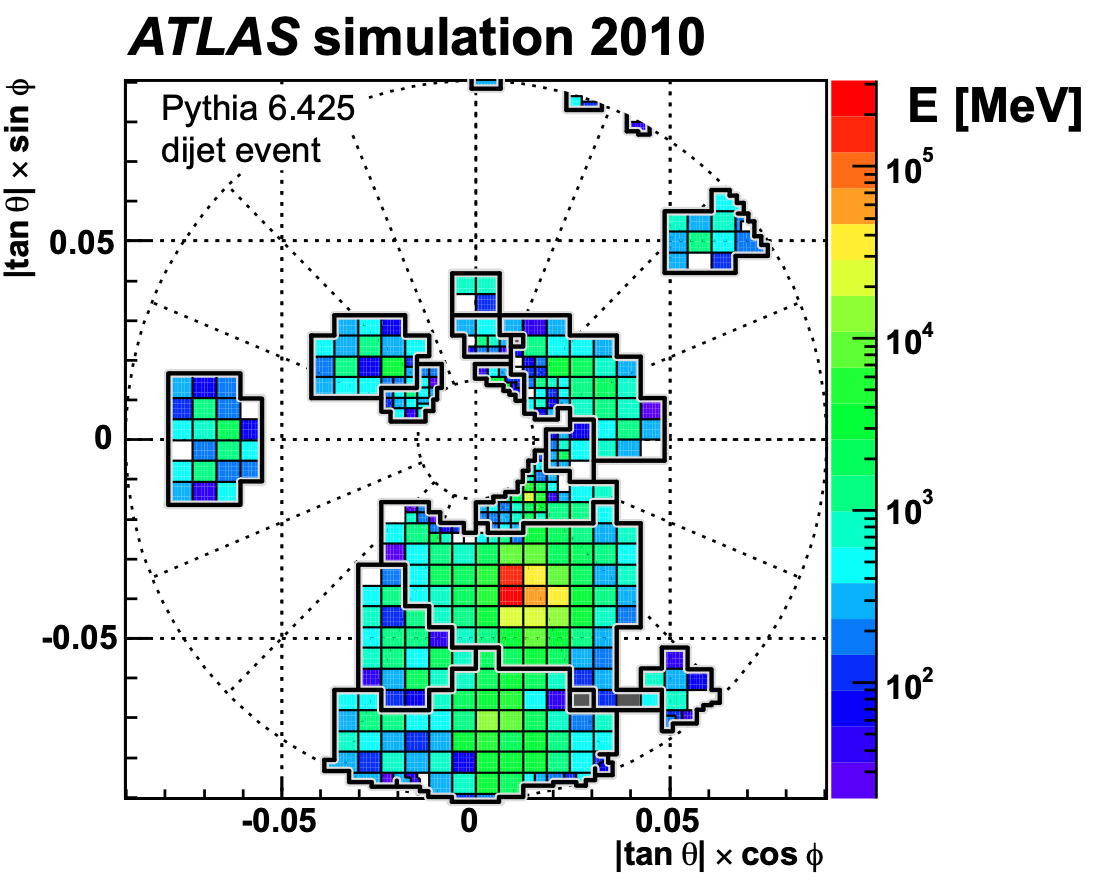
\includegraphics[width=0.7\textwidth]{src/img/topocluster.png}
    \caption{Example of clusters found by the Topocluster algorithm \cite{topocluster}. Black lines separate clusters.}
    \label{fig:topocluster}
\end{figure}

Apart from topo-clusters, the \PFa also uses track information from the inner detector.
The main improvement of the \PFa is the removal of double counting of energy in multiple clusters and putting them together as an energy shower.
A flow chart of the \PFa is shown in \cref{fig:pfo}.
\begin{figure}[ht]
    \centering
    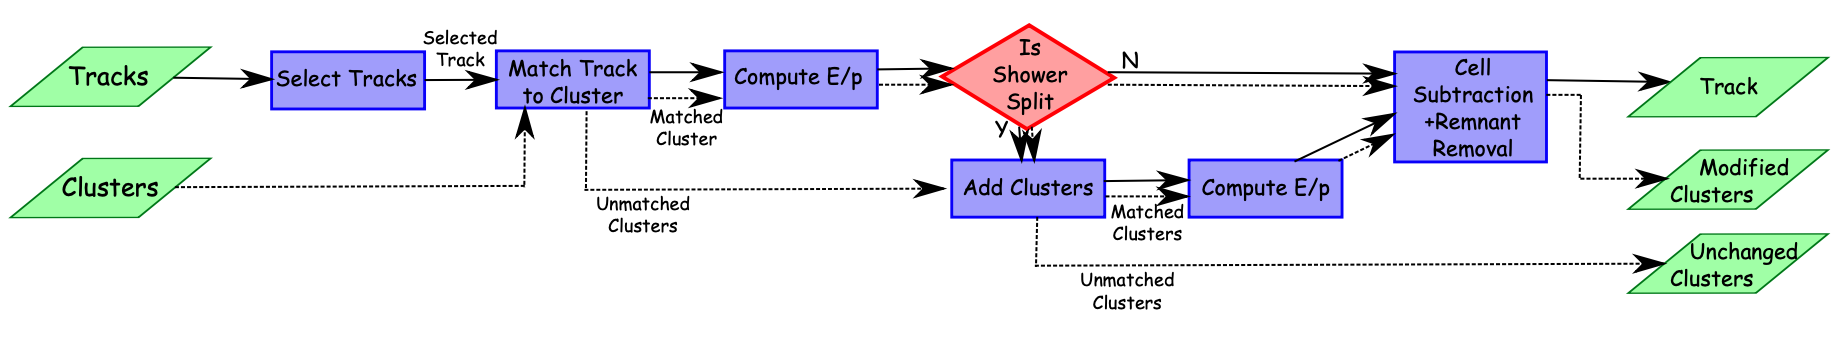
\includegraphics[width=1.\textwidth]{src/img/PF_algorithm.png}
    \caption{Flow chart of the Particle Flow algorithm \cite{PFO}.}
    \label{fig:pfo}
\end{figure}

The object construction procedure is as follows:
\begin{enumerate}
    \item The \PFa \textbf{starts} with the topo-clusters and tracks.
    \item Single \textbf{track is matched} to a single topo-cluster.
    \item \textbf{Energy} of the track and the topo-cluster \textbf{is calculated}.
    \item If the track's energy is larger than the energy of the topo-cluster, a \textbf{new topo-cluster is added} to the list of topo-clusters.
    \item The \textbf{energy} of the list of topo-cluster \textbf{is updated}.
    \item This is \textbf{repeated until} the \textbf{track energy matches} the energy of the list of \textbf{topo-clusters}.
    \item When energy matches, the \textbf{energy} from the list \textbf{of topo-clusters is subtracted} from the whole calorimeter energy, and remnants are removed.
    \item The output of the \PFa is a \textbf{list of topo-clusters and tracks}.
\end{enumerate}

Energy showers used for jet reconstruction are an ensemble of matched topo-clusters and tracks assigned to hard-scattered objects from the primary vertex. 
Note that tracks are assigned only to charged particles with $|\eta| < 2.5$ (tracker position), and only topo-clusters are assigned to neutral particles.
We will refer to elements of topo-cluster and track ensemble as \PFOs. 

\section{Pile-up}
\label{sec:pileup}
\emph{Pile-up} refers to particles created in interactions, not from the primary, hard interaction.
As particles come in bunches, scattering can happen between whole bunches, creating other particles.
The important scatter tagged by the trigger is clouded by pile-up particles, creating another background on top of the electronics.
The Topocluster algorithm searches for clusters on top of the pile-up, meaning that the noise $\sigma$ also contains pile-up particles.

In this context, it is good to introduce variables modeling the pile-up \cite{jvt}.
Specifically, jet-vertex-fraction JVF, corrected JVT corrJVT, momentum fraction originated from primary vertex $R_{\pT}$, jet-vertex-tagger JVT, and forward jet-vertex-tagger fJVT.
\green{The primary vertex has the largest sum of squares of transverse momenta of associated tracks.} 
\begin{description}
     
    \item[The jet-vertex-fraction JVF] is a fraction of the jet \green{transverse} momentum originating from the primary vertex (1st vertex is a shortcut for primary vertex, and 2nd vertex is a shortcut for secondary vertex)
    \begin{equation}
        \label{eq:jvf}
    \text{JVF} = \frac{\sum_{\text{track} \in \text{1st vertex}} \pT^{\text{track}}}{\sum_{\text{track} \in \text{1st vertex}} \pT^{\text{track}} + \sum_{\text{track} \in \text{2nd verticies}} \pT^{\text{track}}},
    \end{equation}
    where $\pT^{\text{track}}$ is the transverse momentum of the track. 
    
    \item[The corrected JVT corrJVT] is a variable that corrects the JVF for the linear increase of pile-up $\pT$ in jet wrt. the total pile-up in an event
    \begin{equation}
        \label{eq:corr_jvf}
        \text{corrJVF} = \frac{\sum_{\text{track} \in \text{1st vertex}} \pT^{\text{track}}}{\sum_{\text{track} \in \text{1st vertex}} \pT^{\text{track}} + \frac{\sum_{\text{track} \in \text{2nd verticies}} \pT^{\text{track}}}{k\cdot N^{\text{track}}_{\text{pile-up}}}},
    \end{equation}
    where $k$ is a constant (usually $k=0.01$), and $N^{\text{track}}_{\text{pile-up}}$ is the total number of pile-up tracks in the event.
    
    
    \item[The variable $R_{\pT}$] is a fraction of the \green{transverse} jet momentum originating from the primary vertex
    \begin{equation}
        \label{eq:rpt}
        R_{\pT} = \frac{\sum_{\text{track} \in \text{1st vertex}} \pT^{\text{track}}}{\pT^{\text{jet}}},
    \end{equation}
    where $\pT^{\text{jet}}$ is the transverse momentum of the whole jet (including topo-clusters).

    \item[The jet-vertex-tagger JVT] is a discriminant calculated from corrJVF and $R_{\pT}$ using \kNN algorithm in two-dimensional corrJVT-$R_{\pT}$ plane. 
    It assigns a number between 0 and 1, where 0 is a pile-up, and 1 is a primary vertex scatter.

    \item[The forward jet-vertex-tagger fJVT] \cite{fjvt} is a variable assigned to forward jets that do not have any track assigned to them given as a normalized projection 
    \begin{equation}
        \label{eq:fjvt}
        \text{fJVT} = \max_{\text{2nd verticies}}{\frac{\textbf{p}^{\text{miss}}_{\text{T, 2nd vertex}} \cdot \textbf{p}_{\text{T}}^{\text{forward jet}}}{|\textbf{p}_{\text{T}}^{\text{forward jet}}|^2}},
    \end{equation}
    where $\textbf{p}_{\text{T}}^{\text{forward jet}}$ is the two-dimensional transverse momentum vector of a forward jet (no tracks assigned), and $\textbf{p}_{\text{T, 2nd vertex}}^{\text{miss}}$ is given by
    \begin{equation}
        \textbf{p}_{\text{T, 2nd vertex}}^{\text{miss}} = -\frac12\left(\sum_{\text{track} \in \text{2nd vertex}} k\textbf{p}_{\text{T}}^{\text{track}} 
        + \sum_{\text{jet} \in \text{2nd vertex} }\textbf{p}_{\text{T}}^{\text{jet}}\right),
    \end{equation}
    where $k$ is a constant (usually $k=2.5$), and $\textbf{p}_{\text{T}}^{\text{track}}$ and $\textbf{p}_{\text{T}}^{\text{jet}}$ are the two-dimensional transverse momentum vectors of tracks and jets assigned to a 2nd vertex, respectively.
\end{description}

It is necessary to emphasize that the momenta $\pT^{\text{track}}$ are calculated from the tracks, not the \PFOs because the Topocluster algorithm cannot assign a vertex.
If a jet has no track assigned, JVF, corrJVF, and JVT are all set to -1.
Jets with JVT$< 0$ are considered as pile-up (passJVT=0), and similarly for fJVT$<0$ (passfJVT=0).\footnote{\green{Jets are also required to have \texttt{Timing}$<10$ ns to pass the fJVT (passfJVT=1). See \cref{ch:app_high_level_variables} for the description of \texttt{Timing}.}}

Another vital variable describing pile-up is the \textbf{average expected number of interactions per bunch crossing} denoted by $\mu$.

\section{Jet Reconstruction}
\label{sec:jet_reco}
There are two commonly used types of jet reconstruction algorithms: \emph{fixed cone} and \emph{sequential recombination} \cite{jet_reco_rev}.

\textbf{Fixed cone algorithms} are based on the idea of a cone of fixed size, where all objects inside the cone make up the jet.
Examples are SISCone \cite{siscone}, or CellJet \cite{pythia}.
The simple principle goes as follows:
\begin{enumerate}
    \item Start with a given direction, usually the momentum direction of the hardest objects.
    \item Construct a cone of fixed size around the direction.
    \item Add all objects inside the cone to the jet and exclude them from further consideration.
    \item Repeat the procedure for the remaining objects.
\end{enumerate}
In case of cones overlapping, they are \green{merged} if the overlapping energy is more than a given threshold (usually 0.5 of total energy).
Jet is split into two if the energy of the overlapping cone is less than a given threshold (usually 0.5 of total energy).

\textbf{Sequential recombination algorithms} are based on clustering jets by some metric, 'distance'.
The general form of the common metric $d_{ij}$ between two object, and reference (\emph{beam}) distance $d_{i\text{B}}$ are given by \cite{antikt}
\begin{equation}
    \label{eq:kt_distance}
    d_{ij} = \min{(p_{\text{T}, i}^{2p}, p_{\text{T}, j}^{2p})} \frac{\Delta^2_{ij}}{R^2}, \quad d_{i\text{B}} = p_{\text{T}, i}^{2p},
\end{equation}
where $p_{\text{T}, i}$ and $p_{\text{T}, j}$ are the transverse momenta of the objects $i$ and $j$, $\Delta^2_{ij} = (y_i - y_j)^2 + (\phi_i - \phi_j)^2$ is the squared radial distance between the constituents (coordinates are as defined in \cref{sec:atlas_coord}), $R$ is the radius parameter, and $p$ is a parameter determining the type of algorithm:
\begin{itemize}
    \item $p=-1$ is the anti-$k_t$ \footnotemark algorithm \cite{antikt},
    \item $p=1$ is the $k_t$ \footnotemark algorithm \cite{kt},
    \item $p=0$ is the Cambridge/Aachen algorithm \cite{Cam_Aachen_alg}.
\end{itemize}
\footnotetext{In the original paper, authors refer to the transverse momentum $\pT$ as $k_t$. Anti-$k_t$ is the reciprocal transverse momentum.}
The algorithm is as follows \cite{antikt}:
\begin{enumerate}
    \item Start with the hardest object and call it an \emph{entity}.
    \item Calculate $d_{ij}$ between entity $i$ and object $j$.
    \item If $d_{ij} < d_{i\text{B}}$, add object $j$ to the entity $i$ (add their 4-momenta) and continue with the next object, going back to step 2.
    \item Else call the entity $i$ a jet and exclude it from further consideration.
    \item Continue until all objects are clustered into jets.
\end{enumerate}
An example of clustered jets with various algorithms is shown in \cref{fig:jet_reco}.
\begin{figure}[ht]
    \centering
    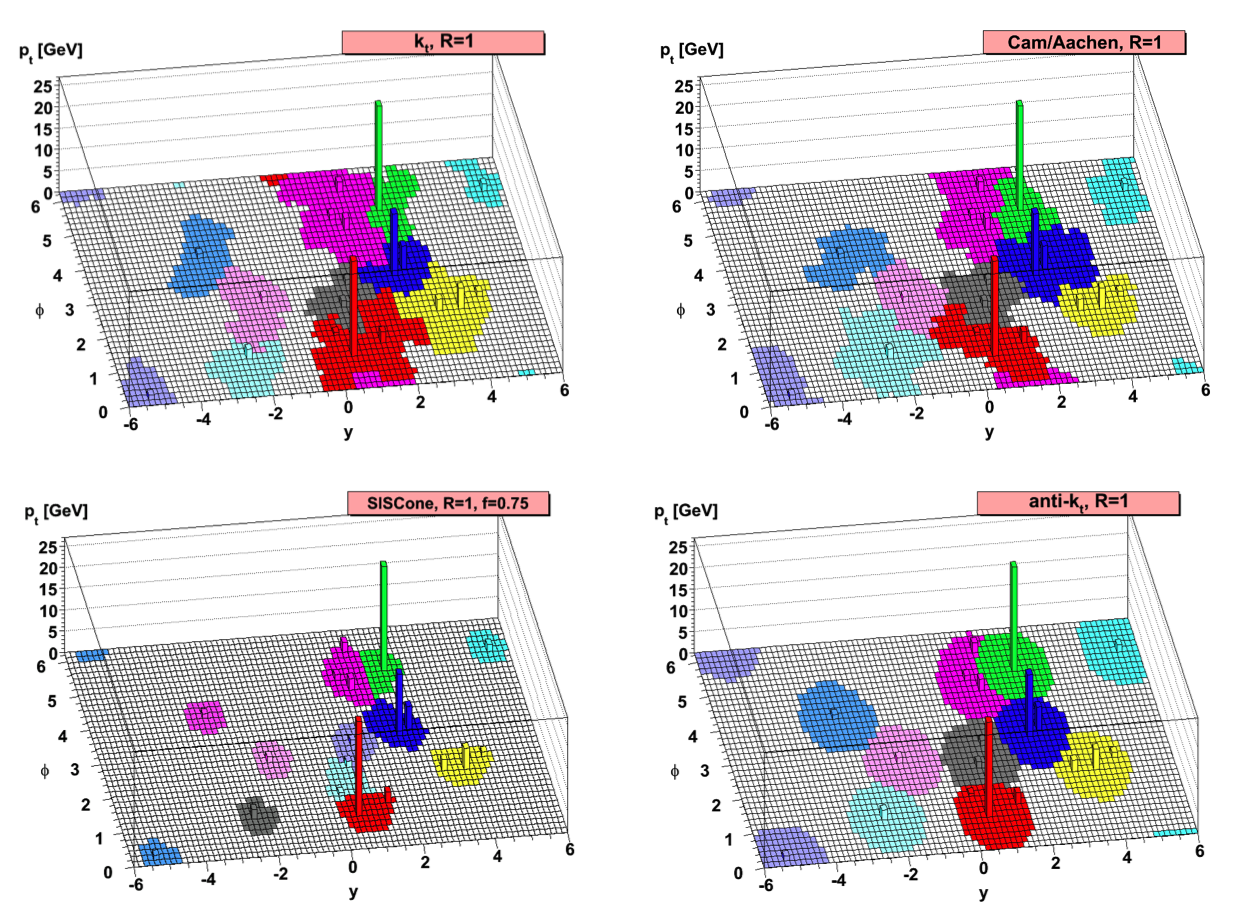
\includegraphics[width=1.\textwidth]{src/img/anitkt.png}
    \caption{Example of clustered jets with various algorithms. The \emph{top left} is the $k_t$ algorithm, the \emph{top right} is the Cambridge/Aachen algorithm, the \emph{bottom left} is the SISCone algorithm, and the \emph{bottom right} is the anti-$k_t$ algorithm.}
    \label{fig:jet_reco}
\end{figure}

In our study, the object referred to in the algorithm descriptions are \PFOs.
The anti-$k_t$ algorithm ($p=-1$) is widely used in the ATLAS community due to its IRC safety (as defined in \cref{def:IRC}) and symmetrical jet shapes. 
We shall use the anti-$k_t$ algorithm with $R=0.4$ for all jet reconstructions.

